\documentclass[12pt]{article}
\usepackage[margin=3cm]{geometry}
\usepackage[utf8]{inputenc}
\usepackage{indentfirst}
\usepackage{amsmath}
\usepackage{fancyhdr}
\usepackage{algorithm}
\usepackage{graphicx}
\usepackage[noend]{algpseudocode}

\fancyhf{}
\pagestyle{fancy}


\renewcommand{\headrulewidth}{0pt}
\renewcommand{\footrulewidth}{1pt}
\renewcommand\footnoterule{}

\rfoot{\thepage}
\lfoot{Afonso Gonçalves, Daniel Seara}


\begin{document}

\title{Análise e Síntese de Algoritmos - 1º Projeto}
\author{Grupo 16 \\ Afonso Gonçalves - 89399 \\ Daniel Seara - 89427}
\date{}
\maketitle


\thispagestyle{fancy}



\section{Introdução}
    O primeiro projeto da cadeira de ASA teve como objetivo executar uma auditoria a uma 
    rede. Esta rede poderá estar dividida em sub-redes, sendo que temos de realizar a 
    auditoria a todas elas. Para tal é necessário calcular que routers da rede, ao serem 
    desligados, aumentariam o número de sub-redes.
    \par
    O Input é dado com M+2 linhas. A primeira indica o número de routers da rede, a segunda 
    o número de ligações entre eles (M) e as restantes representam as ligações (bidirecionais) 
    entre estes, indicando os IDs dos routers em causa.
    \par
    O Output é constituìdo por 4 linhas com, respetivamente, o número de sub-redes da
    rede fornecida, uma sequência ordenada do maior ID de cada subrede, o número de routers 
    que quebram a sub-rede e o número da maior sub-rede formada pela remoção desses routers.
    \par
\section{Descrição da Solução}
    % Linguagem utilizada
    \par
    Decidimos usar a linguagem C++ para a resolução deste problema,
    por ser uma linguagem eficiente, por ter uma boa biblioteca de estruturas de dados 
    que consideramos necessário e ainda por constituir um desafio começar a trabalhar 
    com uma nova linguagem, tão usada e potente nos dias de hoje.

    % Contrução da Solução
    \par
    Identificámos que este problema pode ser resolvido como um problema de grafos:
    Cada router é representado por um vértice e as ligações entre estes pelas respetivas 
    arestas. Os routers que podem quebrar a rede são os vértices de corte ($AP$)
    do grafo e as sub-redes os seus subgrafos.
    \par\bigskip
    Começámos por desenhar um algoritmo que identificava as pontes do grafo, uma vez
    que, removendo pelo menos um dos vértices onde esse arco incide, criaríamos novos 
    subgrafos. Teríamos especial atenção aos vértices que apenas tivessem uma aresta,
    pois a sua remoção não aumentaria o número de subgrafos. Esta abordagem não contempla
    os vértices de articulação que não formam pontes, por isso mudámos de estratégia.
    \par
    Em aula teórica e com alguma pesquisa na internet\cite{geeksforgeeks, hackerearth}
    , aprendemos que o algoritmo de 
    Tarjan permite encontrar os $AP$'s dos grafos. Como esse algoritmo executa uma DFS, 
    seria possível calcular simultaneamente o número de sub-redes do grafo. Para além disso,
    ao visitar cada subgrafo de uma vez, conseguimos também saber o maior ID que lhe pertence.
    \par
    Numa nova iteração do algoritmo, passámos a percorrer os vértices por ordem decrescente de 
    ID, uma vez que estes serão os maiores do respetivo subgrafo. Deste modo, obtemos ainda os 
    ID's máximos de cada subgrafo por ordem decrescente, não sendo necessário ordená-los.
    \par
    Para calcular o número de vértices do maior subgrafo resultante da 
    remoção de todos os vértices críticos encontrados, começámos por  
    remover todos os $AP$'s e as suas arestas e executar uma DFS.
    Rapidamente nos apercebemos que seria uma solução demasiado cara para o efeito: O uso de uma
    flag que indicasse em tempo constante se um vértice é um $AP$ permite ignorá-lo durante a DFS,
    como se tivesse sido removido.
    
    % teoria de grafos
    \par\bigskip
    Com base na teoria de Grafos, sabemos também que é impossível para um grafo completo ter 
    $AP$'s. Desse modo, qualquer grafo com $V$ vértices e 
    \begin{small}$\dfrac{V(V-1)}{2}$\end{small} arestas
    terá necessariamente um subgrafo com ID igual a V e não terá pontos de articulação
    (pela natureza do problema, supomos que não há mais do que uma aresta entre dois vértices
    nem arestas de um vértice para si próprio).
\section{Estruturas de dados empregues}
    \par
    Como neste algoritmo apenas será preciso inserir arestas e iterar por todas as 
    adjacências dos vértices (sem procura), optámos por poupar em memória e representar o 
    grafo usando um array de listas simplesmente ligadas ($\textbf{std::forward\_list\textless int\textgreater*}$). 
    Para minimizar a complexidade, a inserção de novas arestas será sempre feita no início e a 
    iteração do início para o fim.
    \par
    Visto que cada vértice tem um ID, é possível haver acesso à informação necessária para a 
    execução do algoritmo em tempo constante se ela for guardada em array. Preferimos guardar 
    esses arrays na stack porque a alocação e o acesso a essa memória são mais rápidos. 
    Contudo, para inputs muito grandes, obtivemos $Segmentation Fault$, pelo que um desses 
    arrays teve de ser guardado na heap.
    
\section{Algoritmo \& Análise Teórica} 
    O nosso algoritmo tem complexidade linear, com pior caso \textit{$O(V+E)$} 
    e melhor caso \textit{$\Omega$(1)}:
    \begin{itemize}
        \item Inicialização das estruturas: \textit{O(V)}
        \item \textbf{addEdge():} \textit{O(1)}
        \item \textbf{Ciclo While com artPointFind():} \textit{O(V+E)}
        \begin{itemize}
            \item \textbf{minimum():} \textit{O(1)}
            \item Acesso a índices: \textit{O(1)}
            \item \textbf{list.push\_front():} \textit{O(1)}
        \end{itemize}
        \item \textbf{maxSubGraph():} \textit{O(V+E)}
        \begin{itemize}
            \item \textbf{subGraphSize():} \textit{O(V+E)}
        \end{itemize}
        \item Impressão dos resultados: \textit{O(V)}
    \end{itemize}


\section{Demonstração de Resultados}
O nosso algoritmo passa em todos os 16 testes propostos e nos testes disponibilizados. Apresentamos aqui o gráfico de distibuição de 50 testes com número de vértices entre
os 10000 e os 600000 e o seu tempo de execução. Daqui se prova a linearidade da nossa solução.

\begin{figure}[h]
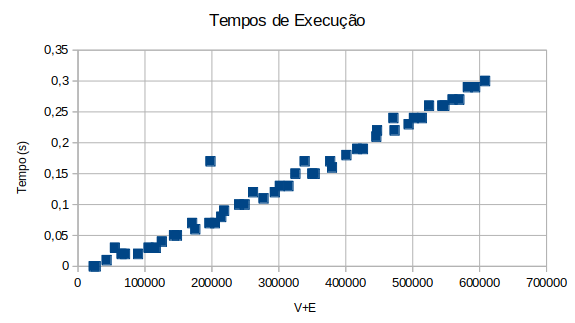
\includegraphics[scale=0.5]{images/VandEGraph}
\centering
\end{figure}

%Para efetuarmos eficientemente o algoritmo precisámos de guardar flags informativas para os 
%vértices. Como eles têm id's numéricos, essas informações podem ser guardadas em vetores e 
%diretamente acedidas, com um baixo custo de memória (a informação teria de ser guardada de 
%qualquer das maneiras). Preferimos guardar esses vetores na stack, para não termos de 
%efetuar chamadas de sistema, que são mais lentas. Contudo, para inputs muito grandes, a 
%stack não é suficientemente grande, pelo que tivemos de guardar um desses vetores na heap, 
%usando a chamada de sistema malloc.

\renewcommand\refname{Referências}
\begin{thebibliography}{9}        
    \bibitem{geeksforgeeks} 
    Articulation Points (or Cut Vertices) in a Graph
    \\\texttt{https://www.geeksforgeeks.org/\\
    articulation-points-or-cut-vertices-in-a-graph/}

    \bibitem{hackerearth} 
    Articulation Points and Bridges
    \\\texttt{https://www.hackerearth.com/\\
    practice/algorithms/graphs/articulation-points-and-bridges/tutorial/}
\end{thebibliography}

\end{document}
